\documentclass[tikz,border=10pt]{standalone}
\usetikzlibrary{calc, arrows, shapes.geometric}
\usepackage{tkz-euclide} %for right angle marker
\usetikzlibrary{backgrounds} % For layering

\begin{document}

%rectangles
\begin{tikzpicture}[scale = 1]
    \def\lengthA{2}
    \def\lengthB{2.5}
    \def\heightA{5}
    \def\heightB{6}
    
    \coordinate (A) at (0,0);
    %rectangle A
    \draw (A) -- ++(0:\lengthA) coordinate(B) -- ++(90:\heightA) coordinate (C) -- ++(180:\lengthA) coordinate[pos=0.5] (M) coordinate (D) -- cycle coordinate[pos=0.5] (N);
    %rectangle B
    \draw (B) -- ++(0:\heightB) -- ++(90:\lengthB) coordinate[pos =0.5] (Q) -- ++(180:\heightB) coordinate[pos = 0.5] (R) -- cycle;

    %labels
    \node at (M) [anchor = south] {$x - 3$};
    \node at (N) [anchor = east] {$2x + 1$};
    \node at (Q) [anchor = west] {4};
    \node at (R) [anchor = south] {$3x - 9$};
\end{tikzpicture}

%Venn diagram
    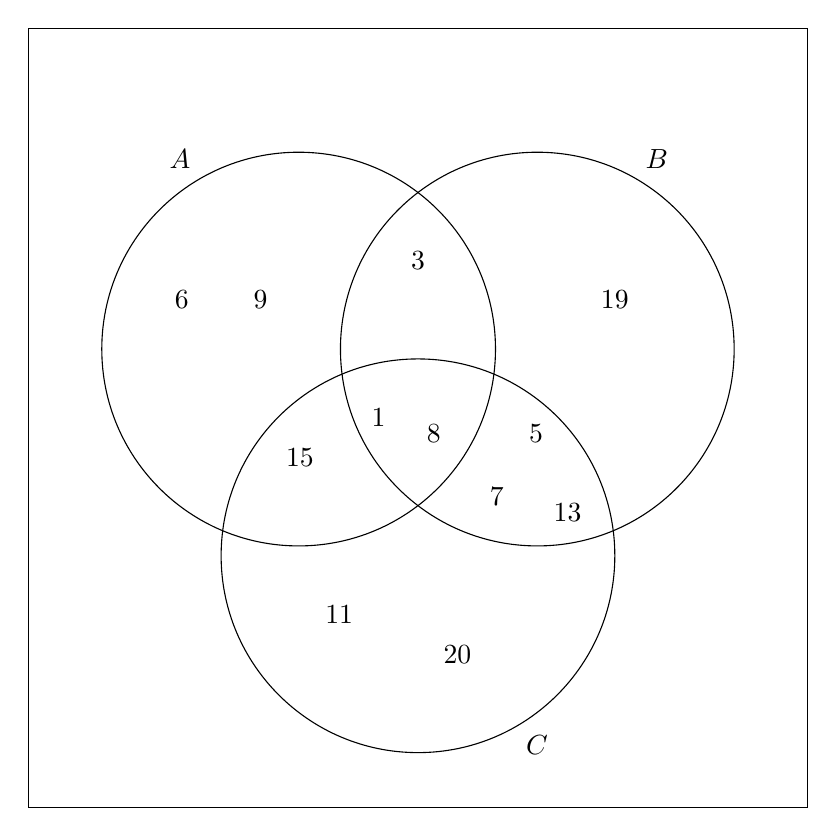
\begin{tikzpicture}[scale = 1]

    \def\firstcircle{(150:1.75cm) circle (2.5cm)}
      \def\secondcircle{(30:1.75cm) circle (2.5cm)}
      \def\thirdcircle{ (-90:1.75cm)circle (2.5cm)}
  
      \path (150:1.75) -- ++(120:2.5) coordinate(K);
      \path (30:1.75) -- ++(60:2.5) coordinate(L);
      \path (-90:1.75) -- ++(-60:2.5) coordinate(M);

      %venn diagram rectangle
      \path (135:7) coordinate (Q);
      \path (45:7) coordinate (R);
      \path (-45:7) coordinate (S);
      \path (-135:7) coordinate (T);
      \draw (Q) -- (R) -- (S) -- (T) -- cycle;

      
      \node at (K) [anchor = south east] {$A$};
      \node at (L) [anchor = south west] {$B$};
      \node at (M) [anchor = north west] {$C$};
      \draw \firstcircle;
      \draw \secondcircle;
      \draw \thirdcircle;

        %elements in set
        \node at (-3, 1.5) [] {6};
        \node at (-2, 1.5) [] {9};
        \node at (0, 2) [] {3};
        \node at (-0.5, 0) [] {1};
        \node at (0.2, -0.2) [] {8};
        \node at (-1.5, -0.5) [] {15};
        \node at (2.5, 1.5) [] {19};
        \node at (1.5, -0.2) [] {5};
        \node at (1, -1) [] {7};
        \node at (1.9, -1.2) [] {13};
        \node at (-1, -2.5) [] {11};
        \node at (0.5, -3) [] {20};
  
    \end{tikzpicture}

%tree diagram
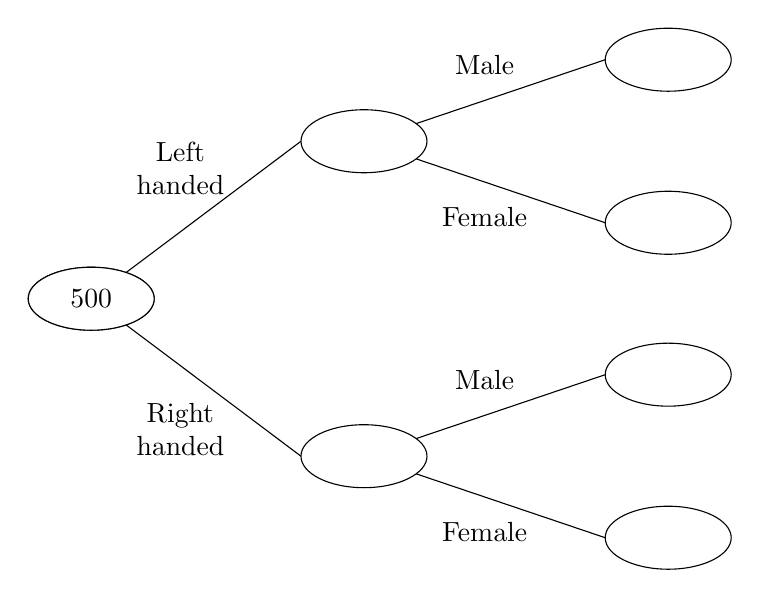
\begin{tikzpicture}
\def\xRadius{0.8}
\def\yRadius{0.4}

\path (0,0) -- ++(30:4cm) coordinate (A);
\path (A) -- ++(180:\xRadius) coordinate (K);
\draw (0,0) -- node[midway, align=center, anchor = south, yshift = 0.2cm, xshift = -0.2cm ]{Left\\handed} (K);
\draw[fill = white] (0,0) ellipse [x radius=\xRadius,y radius=\yRadius];
\path (A) -- ++(15:4cm) coordinate (B);
\path (A) -- ++(-15:4cm) coordinate (C);
\path (B) -- ++(180:\xRadius) coordinate (L);
\path (C) -- ++(180:\xRadius) coordinate (M);
\draw (A) -- node[midway, anchor = south, yshift = 0.2cm] {Male} (L);
\draw (A) -- node[midway, anchor = north, yshift = -0.2cm] {Female} (M) ;
\draw[fill = white] (A) ellipse [x radius = \xRadius, y radius = \yRadius];
\draw[fill = white] (B) ellipse [x radius = \xRadius, y radius = \yRadius];
\draw (C) ellipse [x radius = \xRadius, y radius = \yRadius];


%reflect top branch about xAxis
 \begin{scope}[yscale = -1, xscale = 1]
    \path (0,0) -- ++(30:4cm) coordinate (A);
    \path (A) -- ++(180:\xRadius) coordinate (K);
    \draw (0,0) -- node[midway, align=center, anchor = north, yshift = -0.2cm, xshift = -0.2cm ]{Right\\handed} (K);
    \draw[fill = white] (0,0) ellipse [x radius=\xRadius,y radius=\yRadius];
    \path (A) -- ++(15:4cm) coordinate (B);
    \path (A) -- ++(-15:4cm) coordinate (C);
    \path (B) -- ++(180:\xRadius) coordinate (L);
    \path (C) -- ++(180:\xRadius) coordinate (M);
    \draw (A) -- node[midway, anchor = north, yshift = -0.2cm] {Female} (L);
\draw (A) -- node[midway, anchor = south, yshift = 0.2cm] {Male} (M) ;
    \draw[fill = white] (A) ellipse [x radius = \xRadius, y radius = \yRadius];
    \draw[fill = white] (B) ellipse [x radius = \xRadius, y radius = \yRadius];
    \draw (C) ellipse [x radius = \xRadius, y radius = \yRadius];
 \end{scope}

%label
\node at (0,0) [] {500};
%draw edges

\end{tikzpicture}

%pie chart
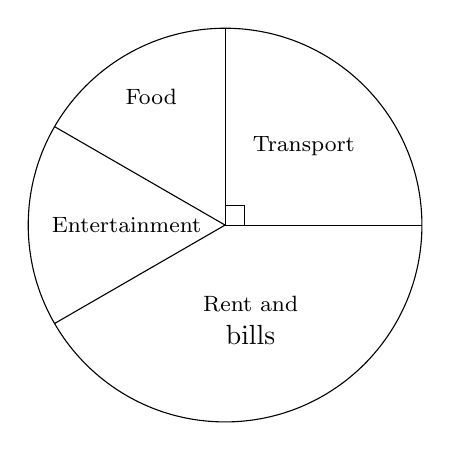
\begin{tikzpicture}
\def\pieRadius{2.5}
\def\transport{90}
\def\food{60}
\def\entertainment{60}
\def\rent{150}

    \coordinate (A) at (0,0);
    \draw (0,0) circle [radius = \pieRadius];
    \draw (0,0) -- ++(0:\pieRadius) coordinate (O);
    \draw (0,0) -- ++(90:\pieRadius) coordinate (T); %Transport
    \draw (0,0) -- ++($(0,0)!1!{\food}:(T)$) coordinate (F); %Food
    \draw (0,0) -- ++($(0,0)!1!\entertainment:(F)$) coordinate (E); %Entertainment

    \tkzMarkRightAngle[size=.25](O,A,T);

    %Labels
    \node at (0.4 * \pieRadius, 0.4* \pieRadius) [] {\footnotesize Transport};
    \path (A) -- ++($(A)!0.75!{0.5* \food}:(T)$) coordinate (P);
    \path (A) -- ++($(A)!0.5!{0.5* \entertainment}:(F)$) coordinate (Q);
    \path (A) -- ++($(A)!0.5!{0.5* \rent}:(E)$) coordinate (R);
    \node at (P) [] {\footnotesize Food};
    \node at (Q) [] {\footnotesize Entertainment};
    \node at (R) [align = center] {\footnotesize Rent and \\ bills};
\end{tikzpicture}

%Number Line
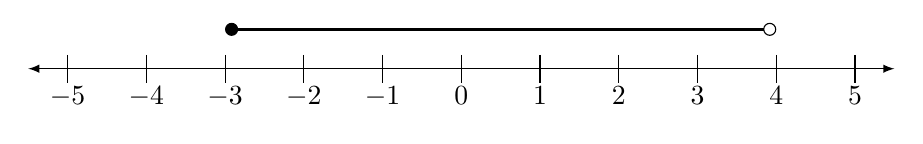
\begin{tikzpicture}

\draw[latex-latex] (-5.5,0) -- (5.5,0) ; %edit here for the axis
\foreach \x in {-5,-4,-3,-2,-1,0,1,2,3,4,5} % edit here for the vertical lines
\draw[shift={(\x,0)},color=black] (0pt,5pt) -- (0pt,-5pt);
\foreach \x in {-5,-4,-3,-2,-1,0,1,2,3,4,5} % edit here for the numbers
\draw[shift={(\x,0)},color=black] (0pt,0pt) -- (0pt,-3pt) node[below] 
{$\x$};
\draw[*-o] (-3,0.5) -- (4,0.5); % use -o for non-inclusive
\draw[very thick] (-2.9,0.5) -- (3.85,0.5);

\end{tikzpicture}

%Number Line 2
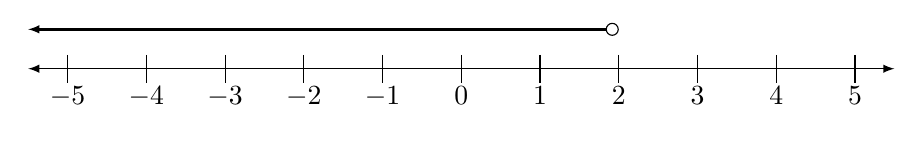
\begin{tikzpicture}

\draw[latex-latex] (-5.5,0) -- (5.5,0) ; %edit here for the axis
\foreach \x in {-5,-4,-3,-2,-1,0,1,2,3,4,5} % edit here for the vertical lines
\draw[shift={(\x,0)},color=black] (0pt,5pt) -- (0pt,-5pt);
\foreach \x in {-5,-4,-3,-2,-1,0,1,2,3,4,5} % edit here for the numbers
\draw[shift={(\x,0)},color=black] (0pt,0pt) -- (0pt,-3pt) node[below] 
{$\x$};
\draw[latex-o] (-5.5,0.5) -- (2,0.5); % use -o for non-inclusive
\draw[very thick] (-5.4,0.5) -- (1.85,0.5);

\end{tikzpicture}

%Probability spinner Octagon
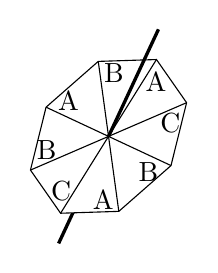
\begin{tikzpicture}
    % Define skewed coordinates
    \coordinate (O) at (0,0);
    \foreach \x in {1,2,...,8}{
        % Angle calculation for octagon vertices
        \pgfmathsetmacro{\angle}{45*\x+22.5+30} % 22.5 is the starting angle, 30 is additional rotation
        % Coordinate calculation with skewing for 3D effect
        \pgfmathsetmacro{\xcoord}{cos(\angle)}
        \pgfmathsetmacro{\ycoord}{sin(\angle) + 0.3*cos(\angle)}
        \coordinate (P\x) at (\xcoord, \ycoord);
    }
    
    % Draw the line appearing from bottom in the background layer
    \begin{pgfonlayer}{background}
        % Draw the bottom part of the pin, covered by the octagon
    \draw[ very thick] (O) -- ++(245:1.5cm); % Pin extending downwards
    \end{pgfonlayer}

     % Draw the skewed octagon
        \draw[fill=white] (P1) \foreach \x in {2,...,8}{-- (P\x)} -- cycle;

        % Draw lines to the center and label triangles
        \foreach \x [count=\xi] in {1,2,...,8}{
            \pgfmathtruncatemacro{\nextvertex}{mod(\x,8) + 1}
            \coordinate (Center) at (barycentric cs:P1=1,P2=1,P3=1,P4=1,P5=1,P6=1,P7=1,P8=1);
            \draw (P\x) -- (Center);
            \pgfmathtruncatemacro{\labelindex}{mod(\xi,3)}
            \ifnum\labelindex=0
                \node at ($(Center)!0.6!(P\x)!0.6!(P\nextvertex)$) {C};
            \else
                \ifnum\labelindex=1
                    \node at ($(Center)!0.6!(P\x)!0.6!(P\nextvertex)$) {A};
                \else
                    \node at ($(Center)!0.6!(P\x)!0.6!(P\nextvertex)$) {B};
                \fi
            \fi
        }
        
    % Draw the pin (probability spinner) top part
    \draw[very thick] (O) -- ++(65:1.5cm); % Pin extending upwards
   
\end{tikzpicture}

%probability spinner square
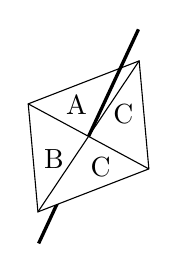
\begin{tikzpicture}
    % Define skewed coordinates for a 3D perspective
    \coordinate (O) at (0,0);
    \foreach \x in {1,2,3,4}{
        \pgfmathsetmacro{\angle}{90*\x-40} % Square vertices angle
        \pgfmathsetmacro{\xcoord}{cos(\angle)}
        \pgfmathsetmacro{\ycoord}{sin(\angle) + 0.3*cos(\angle)}
        \coordinate (P\x) at (\xcoord,\ycoord);
    }

    % Draw the line appearing from bottom in the background layer
    \begin{pgfonlayer}{background}
        % Draw the bottom part of the pin, covered by the square
        \draw[very thick] (O) -- ++(245:1.5cm); % Pin extending downwards
    \end{pgfonlayer}

    % Draw the skewed square
    \draw[fill=white] (P1) \foreach \x in {2,3,4}{-- (P\x)} -- cycle;

    % Draw lines to the center and label triangles
    \foreach \x [count=\xi] in {1,2,3,4}{
        \pgfmathtruncatemacro{\nextvertex}{mod(\x,4) + 1}
        \draw (P\x) -- (O);
        % Labeling the triangles
        \ifnum\xi=1
            \node at ($(O)!0.4!(P\x)!0.4!(P\nextvertex)$) {A};
        \else
            \ifnum\xi=2
                \node at ($(O)!0.4!(P\x)!0.4!(P\nextvertex)$) {B};
            \else
                \ifnum\xi=3
                    \node at ($(O)!0.4!(P\x)!0.4!(P\nextvertex)$) {C};
                \else
                    \node at ($(O)!0.4!(P\x)!0.4!(P\nextvertex)$) {C};
                \fi
            \fi
        \fi
    }

    % Draw the pin (probability spinner) top part
    \draw[very thick] (O) -- ++(65:1.5cm); % Pin extending upwards
\end{tikzpicture}

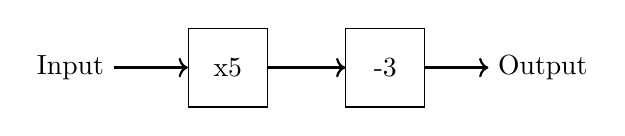
\begin{tikzpicture}

    % Draw nodes and arrows
    \node (input) at (0,0) {Input};
    \node[draw, rectangle, align=center, minimum width=1cm, minimum height=1cm] (multiply) at (2,0) {x5};
    \node[draw, rectangle, align=center, minimum width=1cm, minimum height=1cm] (subtract) at (4,0) {-3};
    \node (output) at (6,0) {Output};

    \draw[->, thick] (input) -- (multiply);
    \draw[->, thick] (multiply) -- (subtract);
    \draw[->, thick] (subtract) -- (output);

\end{tikzpicture}
\end{document}